\chapter{Thermodynamics and Finite Size Scaling}

	In this Chapter,  a comparison between mean and exact thermodynamic variables along with the estimation of the Curie temperature for the infinite lattice.

\section{Avoiding Overflow in Thermodynamic Computations}

	Extracting thermodynamic information from the JDoS can be a difficult process, specially when trying to study large systems. Although the formulas from Chapter 1 are easy to understand, the problem arrives when trying to actually compute the partition function and consequent Boltzmann factors for the ensemble average variables. For large systems, the values from the JDoS are very large, for instance, for an L16 SS Ising system, some of the values of the JDoS are of the order $10^{74}$. We can not keep summing and multiplying these values to compute $Z$, since we run into overflow errors. For low temperatures we run into the same error, since the exponential gets very large. Instead we have to work with the logarithms of these functions to extract the thermodynamics out of the JDoS. We can use the following observation,
\begin{equation}
	\ln \left(  \sum_i a_i \right) = \ln(a_0) + \ln\left( 1 + \sum_{i \neq 0} \frac{a_i}{a_0} \right)
\end{equation}

\section{Mean and Exact Thermodynamic Variables}

	As previously mentioned in Chapter 1, we can calculate thermodynamic variables from the JDoS in two different ways. One by calculating the ensemble average of the energy and magnetization and then the average heat capacity and another one by computing the Helmholtz free energy and using the energy minimization principle we can compute the exact energy, magnetization and heat capacity. For three different system sizes, there computations can be seen in Figure 5.1, along with the exact solution by Onsager. 
	
	We would expect that these two ways of computing the same variable would yield similar results. 

\begin{figure}[h]
	\centering
	\subfigure[]{
		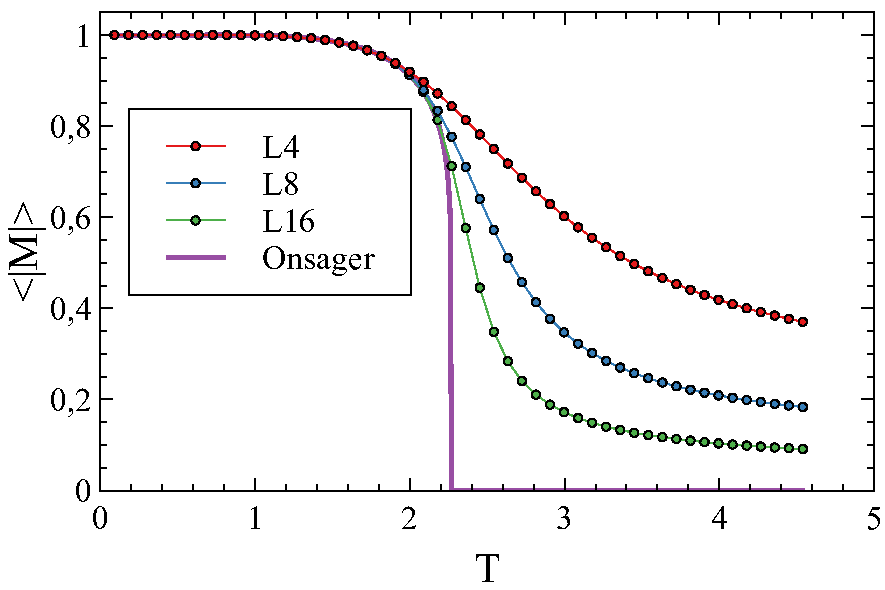
\includegraphics[scale=0.49]{thermodynamics/thermodynamics_finite_size_03.pdf}
	}	
	\subfigure[]{
		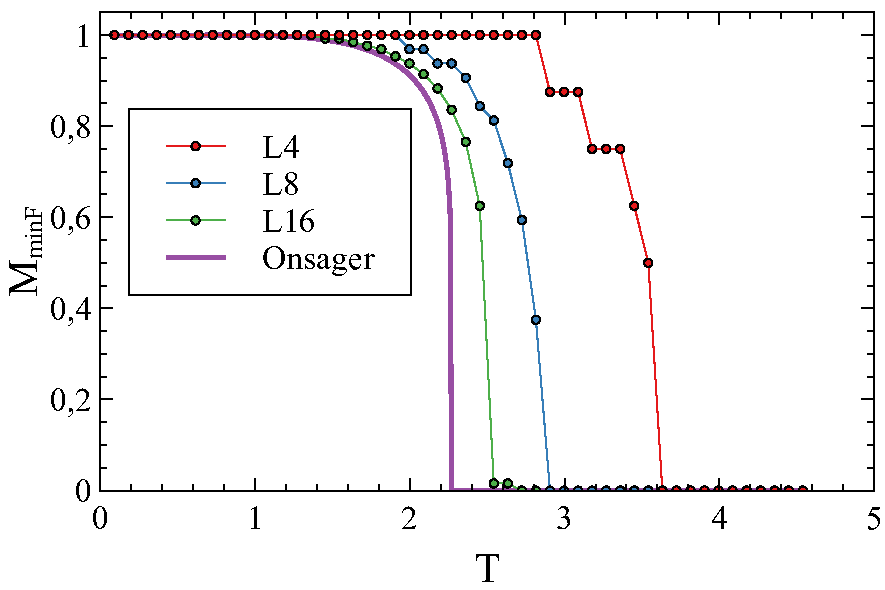
\includegraphics[scale=0.49]{thermodynamics/thermodynamics_finite_size_02.pdf}
	}	
	
	\subfigure[]{
		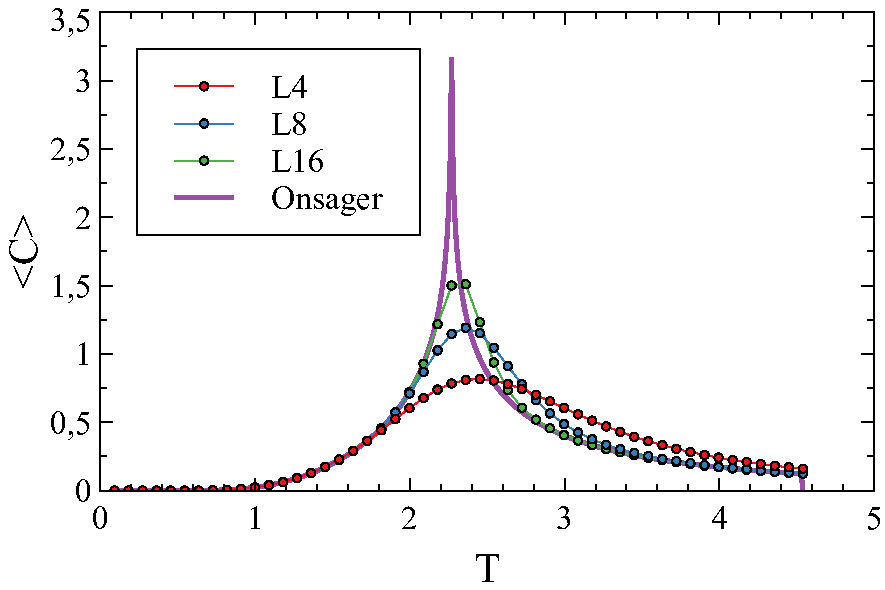
\includegraphics[scale=0.49]{thermodynamics/thermodynamics_finite_size_05.pdf}
	}	
	\subfigure[]{
		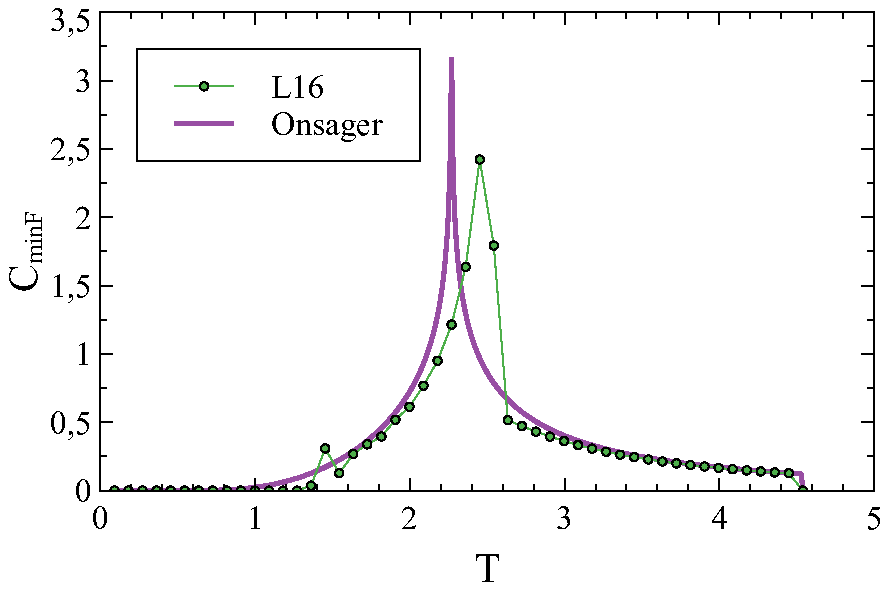
\includegraphics[scale=0.49]{thermodynamics/thermodynamics_finite_size_04.pdf}
	}	
	\label{thermo_4}
	\caption{Thermodynamics for 3 different lattice sizes compared with the exact solution by Onsager.}
\end{figure}


%\begin{figure}[h]
%	\centering
%	\subfigure[]{
%			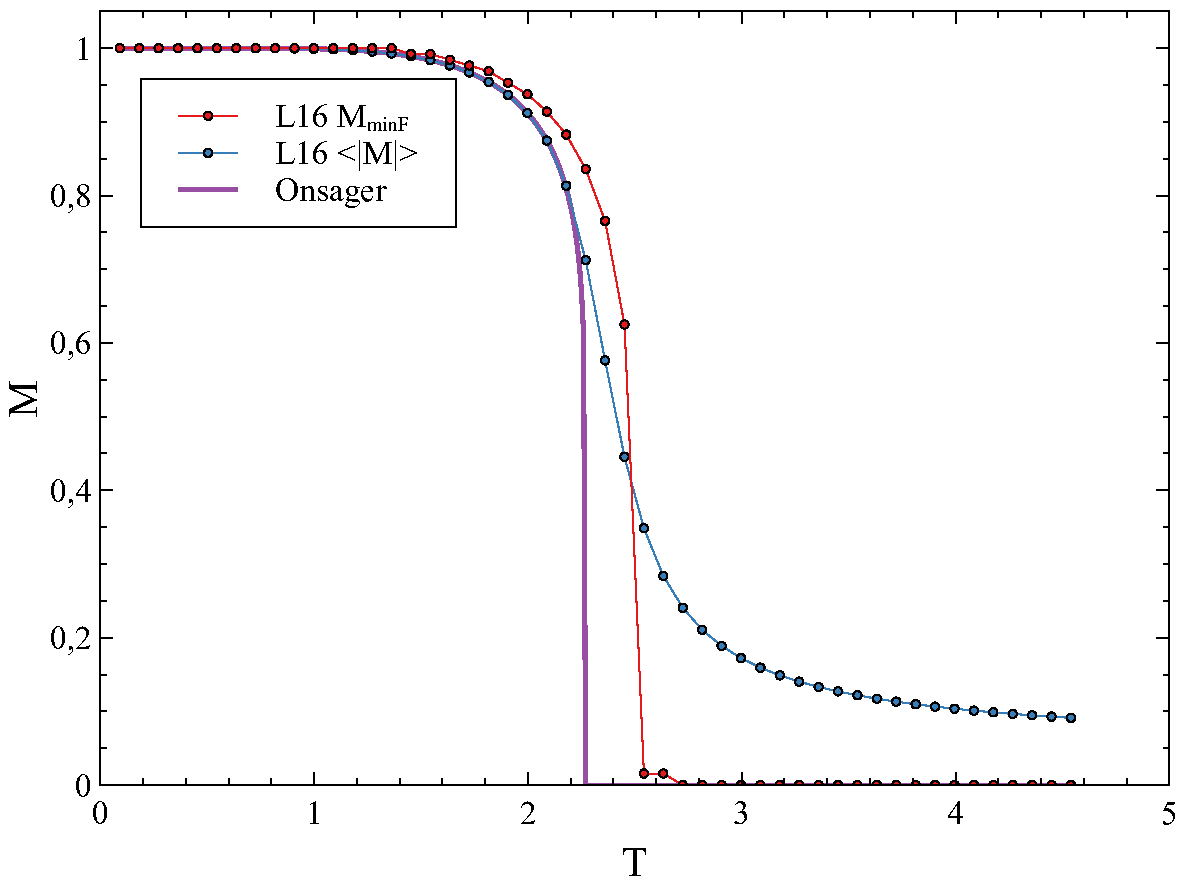
\includegraphics[scale=0.37]{thermodynamics/thermodynamics_finite_size_06.pdf}
%	}
%	\subfigure[]{
%		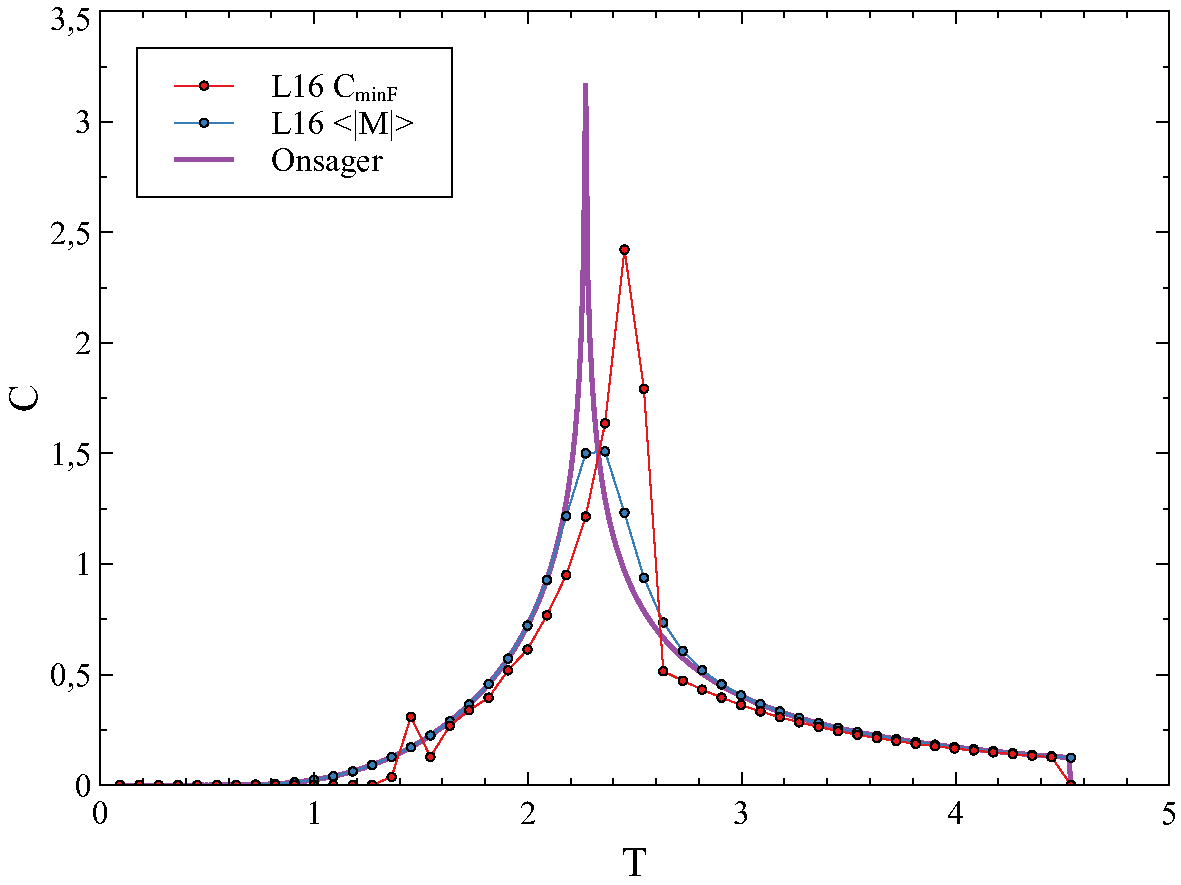
\includegraphics[scale=0.37]{thermodynamics/thermodynamics_finite_size_07.pdf}
%	}
%	
%	\caption{Scheme of how the Flat Scan Sampling works.}
%\end{figure}

\section{Estimating $T_C$ for the Infinite Lattice}

\begin{figure}[h]
	\centering
	\subfigure[]{
		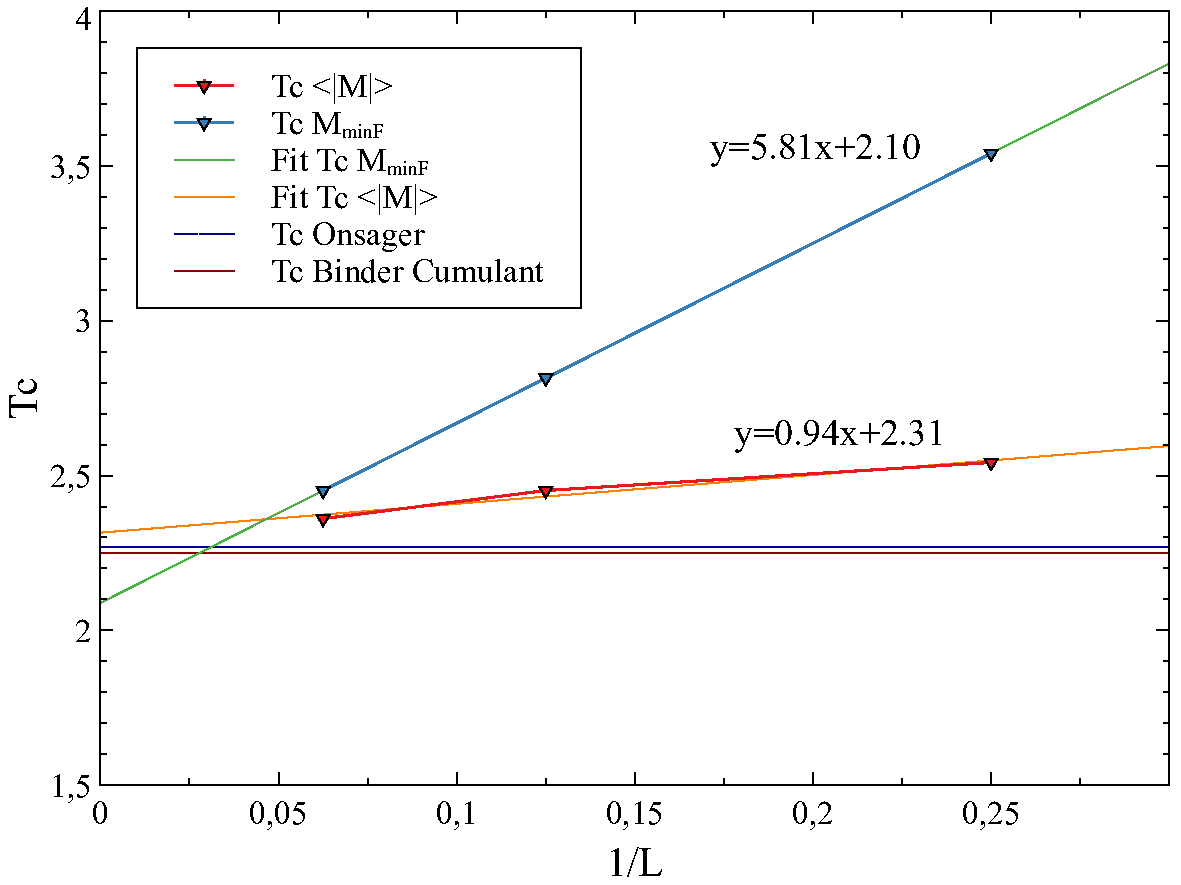
\includegraphics[scale=0.37]{thermodynamics/thermodynamics_finite_size_01.pdf}
	}	
	\subfigure[]{
		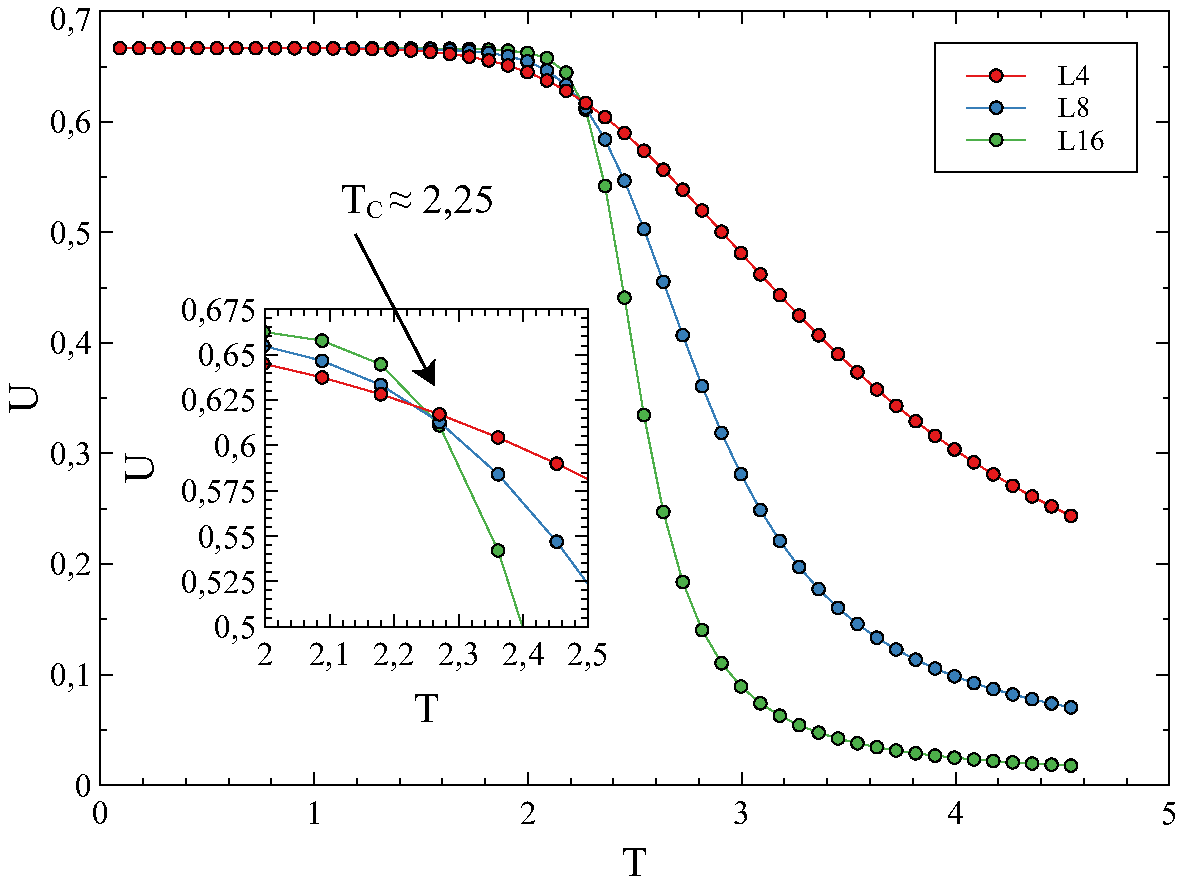
\includegraphics[scale=0.37]{thermodynamics/thermodynamics_finite_size_08.pdf}
	}	
	\caption{Estimation of the $T_C$ for the infinite lattice.}
\end{figure}


